\documentclass{standalone}
\usepackage{tikz}
\usetikzlibrary{patterns}
\usetikzlibrary{positioning}
\usetikzlibrary{patterns, positioning}
\usetikzlibrary{shapes.misc}
\usepackage[outline]{contour}
\contourlength{1.5pt} 
\usepackage[sfdefault]{ClearSans}

\begin{document}
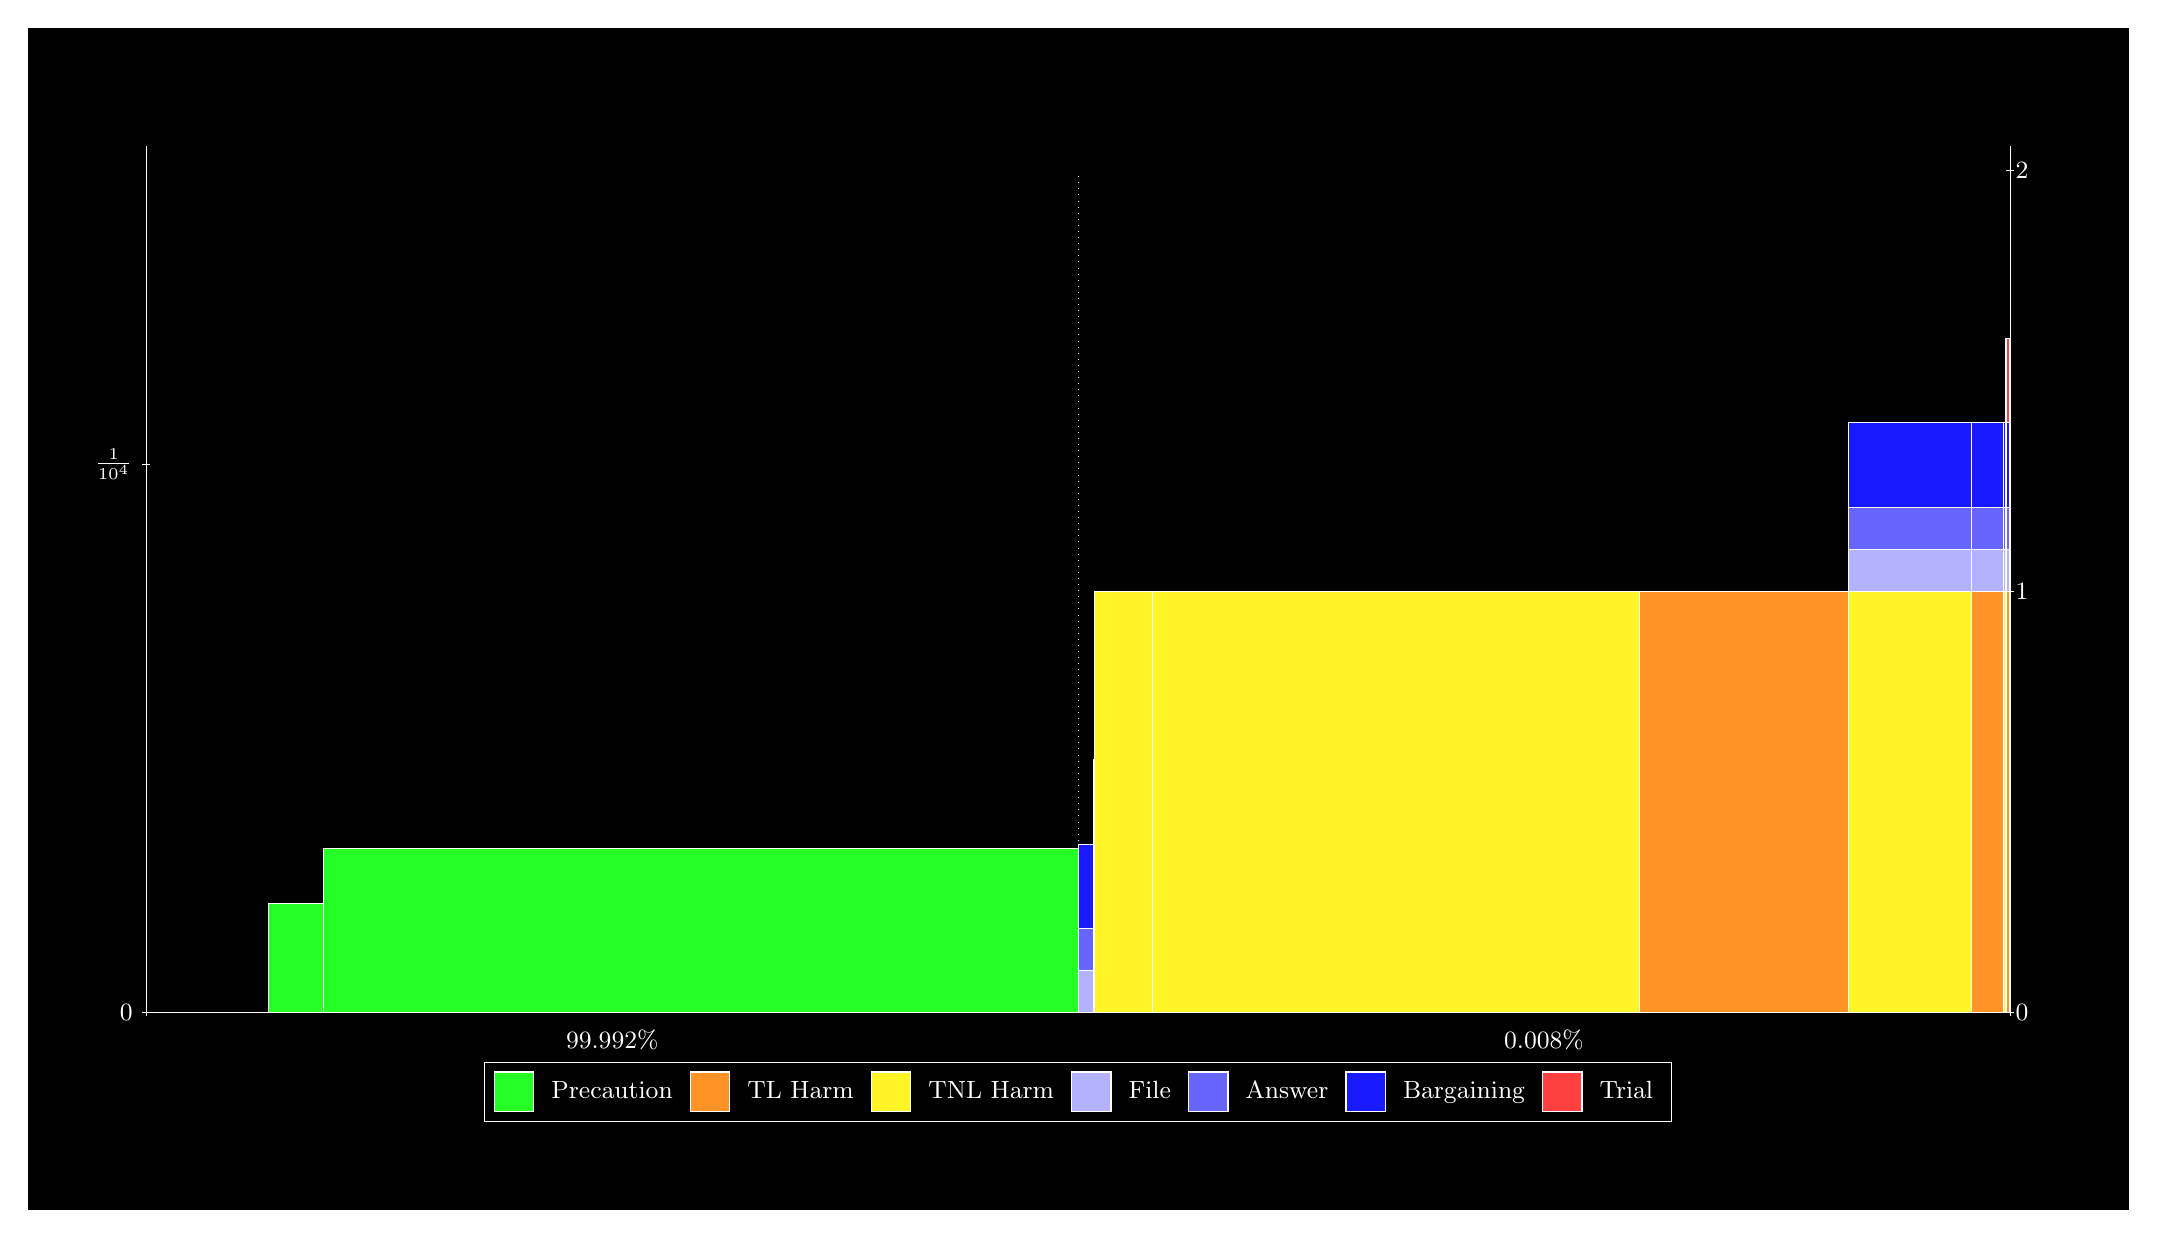
\begin{tikzpicture}
\draw[fill=black] (0,0) rectangle (26.667,15);
\draw[fill=green!85,draw=white,very thin] (3.0469,2.5) rectangle (3.7465,3.8926);
\draw[fill=green!85,draw=white,very thin] (3.7465,2.5) rectangle (13.333,4.5888);
\draw[fill=blue!30,draw=white,very thin] (13.333,2.5) rectangle (13.53,3.035);
\draw[fill=blue!60,draw=white,very thin] (13.333,3.035) rectangle (13.53,3.5699);
\draw[fill=blue!90,draw=white,very thin] (13.333,3.5699) rectangle (13.53,4.6399);
\draw[fill=blue!30,draw=white,very thin] (13.53,2.5) rectangle (13.535,3.035);
\draw[fill=blue!60,draw=white,very thin] (13.53,3.035) rectangle (13.535,3.5699);
\draw[fill=blue!90,draw=white,very thin] (13.53,3.5699) rectangle (13.535,4.6399);
\draw[fill=red!75,draw=white,very thin] (13.53,4.6399) rectangle (13.535,5.7098);
\draw[fill=green!85,draw=white,very thin] (13.535,2.5) rectangle (14.279,2.5001);
\draw[fill=yellow!85,draw=white,very thin] (13.535,2.5001) rectangle (14.279,7.8498);
\draw[fill=green!85,draw=white,very thin] (14.279,2.5) rectangle (20.46,2.5002);
\draw[fill=yellow!85,draw=white,very thin] (14.279,2.5002) rectangle (20.46,7.8498);
\draw[fill=green!85,draw=white,very thin] (20.46,2.5) rectangle (23.114,2.5002);
\draw[fill=orange!85,draw=white,very thin] (20.46,2.5002) rectangle (23.114,7.8498);
\draw[fill=yellow!85,draw=white,very thin] (23.114,2.5) rectangle (24.672,7.8497);
\draw[fill=blue!30,draw=white,very thin] (23.114,7.8497) rectangle (24.672,8.3846);
\draw[fill=blue!60,draw=white,very thin] (23.114,8.3846) rectangle (24.672,8.9196);
\draw[fill=blue!90,draw=white,very thin] (23.114,8.9196) rectangle (24.672,9.9895);
\draw[fill=orange!85,draw=white,very thin] (24.672,2.5) rectangle (25.079,7.8497);
\draw[fill=blue!30,draw=white,very thin] (24.672,7.8497) rectangle (25.079,8.3846);
\draw[fill=blue!60,draw=white,very thin] (24.672,8.3846) rectangle (25.079,8.9196);
\draw[fill=blue!90,draw=white,very thin] (24.672,8.9196) rectangle (25.079,9.9895);
\draw[fill=green!85,draw=white,very thin] (25.079,2.5) rectangle (25.111,2.5001);
\draw[fill=yellow!85,draw=white,very thin] (25.079,2.5001) rectangle (25.111,7.8498);
\draw[fill=blue!30,draw=white,very thin] (25.079,7.8498) rectangle (25.111,8.3847);
\draw[fill=blue!60,draw=white,very thin] (25.079,8.3847) rectangle (25.111,8.9197);
\draw[fill=blue!90,draw=white,very thin] (25.079,8.9197) rectangle (25.111,9.9896);
\draw[fill=green!85,draw=white,very thin] (25.111,2.5) rectangle (25.113,2.5001);
\draw[fill=orange!85,draw=white,very thin] (25.111,2.5001) rectangle (25.113,7.8498);
\draw[fill=blue!30,draw=white,very thin] (25.111,7.8498) rectangle (25.113,8.3847);
\draw[fill=blue!60,draw=white,very thin] (25.111,8.3847) rectangle (25.113,8.9197);
\draw[fill=blue!90,draw=white,very thin] (25.111,8.9197) rectangle (25.113,9.9896);
\draw[fill=yellow!85,draw=white,very thin] (25.113,2.5) rectangle (25.116,7.8497);
\draw[fill=blue!30,draw=white,very thin] (25.113,7.8497) rectangle (25.116,8.3846);
\draw[fill=blue!60,draw=white,very thin] (25.113,8.3846) rectangle (25.116,8.9196);
\draw[fill=blue!90,draw=white,very thin] (25.113,8.9196) rectangle (25.116,9.9895);
\draw[fill=red!75,draw=white,very thin] (25.113,9.9895) rectangle (25.116,11.059);
\draw[fill=orange!85,draw=white,very thin] (25.116,2.5) rectangle (25.16,7.8497);
\draw[fill=blue!30,draw=white,very thin] (25.116,7.8497) rectangle (25.16,8.3846);
\draw[fill=blue!60,draw=white,very thin] (25.116,8.3846) rectangle (25.16,8.9196);
\draw[fill=blue!90,draw=white,very thin] (25.116,8.9196) rectangle (25.16,9.9895);
\draw[fill=red!75,draw=white,very thin] (25.116,9.9895) rectangle (25.16,11.059);
\draw[fill=green!85,draw=white,very thin] (25.16,2.5) rectangle (25.165,2.5001);
\draw[fill=yellow!85,draw=white,very thin] (25.16,2.5001) rectangle (25.165,7.8498);
\draw[fill=blue!30,draw=white,very thin] (25.16,7.8498) rectangle (25.165,8.3847);
\draw[fill=blue!60,draw=white,very thin] (25.16,8.3847) rectangle (25.165,8.9197);
\draw[fill=blue!90,draw=white,very thin] (25.16,8.9197) rectangle (25.165,9.9896);
\draw[fill=red!75,draw=white,very thin] (25.16,9.9896) rectangle (25.165,11.06);
\draw[fill=green!85,draw=white,very thin] (25.165,2.5) rectangle (25.167,2.5001);
\draw[fill=orange!85,draw=white,very thin] (25.165,2.5001) rectangle (25.167,7.8498);
\draw[fill=blue!30,draw=white,very thin] (25.165,7.8498) rectangle (25.167,8.3847);
\draw[fill=blue!60,draw=white,very thin] (25.165,8.3847) rectangle (25.167,8.9197);
\draw[fill=blue!90,draw=white,very thin] (25.165,8.9197) rectangle (25.167,9.9896);
\draw[fill=red!75,draw=white,very thin] (25.165,9.9896) rectangle (25.167,11.06);
\draw[white,very thin] (1.5,2.5) -- (1.5,13.5);
\draw[white,very thin] (1.45,2.5) -- (1.55,2.5);
\node[font=\small,text=white, anchor=east] at (1.45, 2.5) {0};
\draw[white,very thin] (1.45,9.4628) -- (1.55,9.4628);
\node[font=\small,text=white, anchor=east] at (1.45, 9.4628) {$\frac{1}{10^{4}}$};

\draw[white,dotted,very thin] (13.333,2.83) -- (13.333,13.17);
\draw[white,very thin] (25.167,2.5) -- (25.167,13.5);
\draw[white,very thin] (25.117,2.5) -- (25.217,2.5);
\node[font=\small,text=white, anchor=west] at (25.117, 2.5) {0};
\draw[white,very thin] (25.117,7.8497) -- (25.217,7.8497);
\node[font=\small,text=white, anchor=west] at (25.117, 7.8497) {1};
\draw[white,very thin] (25.117,13.199) -- (25.217,13.199);
\node[font=\small,text=white, anchor=west] at (25.117, 13.199) {2};

\draw[white,very thin] (1.5,2.5) -- (25.167,2.5);
\draw[white,very thin] (1.5,2.45) -- (1.5,2.55);
\node[font=\small,text=white, anchor=north] at (1.5, 2.45) {};
\draw[white,very thin] (25.167,2.45) -- (25.167,2.55);
\node[font=\small,text=white, anchor=north] at (25.167, 2.45) {};

\node[font=\small,text=white,anchor=south] at (7.4167, 1.9) {99.992\%};
\node[font=\small,text=white,anchor=south] at (19.25, 1.9) {0.008\%};
\draw (13.3333,2.5) node (B) {};
\begin{scope}[align=center]
\matrix[scale=0.5,draw=white,below=0.5cm of B,nodes={draw},column sep=0.1cm]{
\node[rectangle,draw,minimum width=0.5cm,minimum height=0.5cm,fill=green!85]{}; & \node[draw=none,font=\small,text=white]{Precaution}; &
\node[rectangle,draw,minimum width=0.5cm,minimum height=0.5cm,fill=orange!85]{}; & \node[draw=none,font=\small,text=white]{TL Harm}; &
\node[rectangle,draw,minimum width=0.5cm,minimum height=0.5cm,fill=yellow!85]{}; & \node[draw=none,font=\small,text=white]{TNL Harm}; &
\node[rectangle,draw,minimum width=0.5cm,minimum height=0.5cm,fill=blue!30]{}; & \node[draw=none,font=\small,text=white]{File}; &
\node[rectangle,draw,minimum width=0.5cm,minimum height=0.5cm,fill=blue!60]{}; & \node[draw=none,font=\small,text=white]{Answer}; &
\node[rectangle,draw,minimum width=0.5cm,minimum height=0.5cm,fill=blue!90]{}; & \node[draw=none,font=\small,text=white]{Bargaining}; &
\node[rectangle,draw,minimum width=0.5cm,minimum height=0.5cm,fill=red!75]{}; & \node[draw=none,font=\small,text=white]{Trial}; \\\\
};\end{scope}

\end{tikzpicture}
\end{document}